\documentclass{standalone}
\usepackage{tikz}
\usetikzlibrary{patterns}

\begin{document}
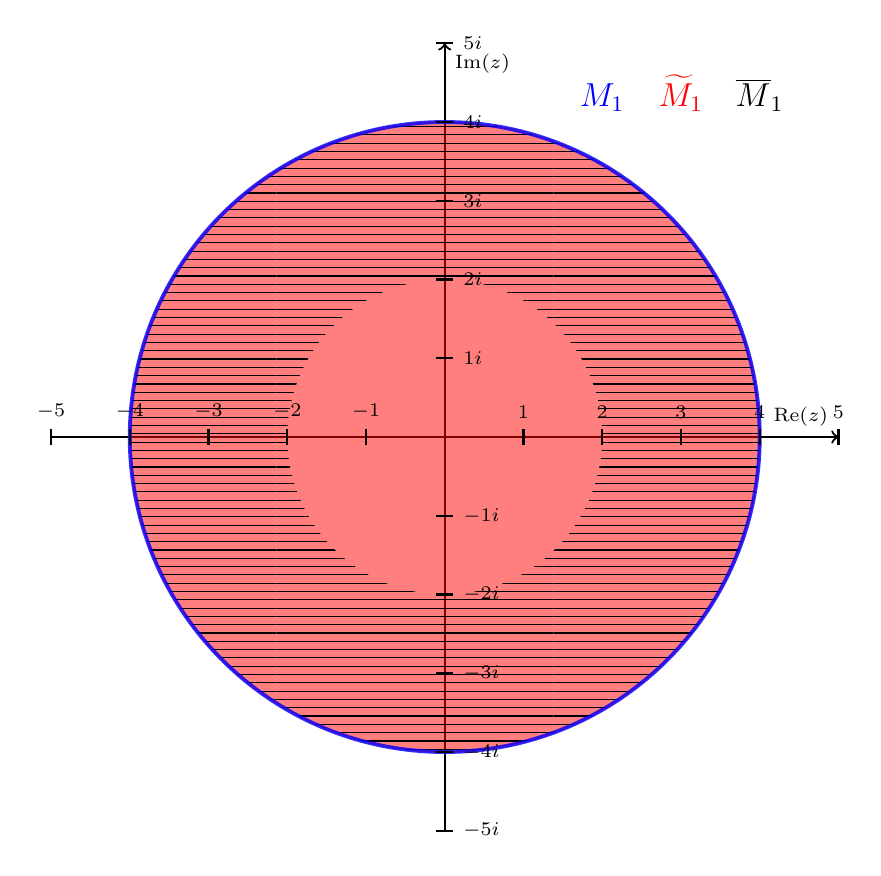
\begin{tikzpicture}
    \begin{scope}[thick,font=\scriptsize]

        \draw [->] (-5,0) -- (5,0) node [above left]  {Re$(z)$};
        \draw [->] (0,-5) -- (0,5) node [below right] {Im$(z)$};

        \path [draw=red,fill=red,opacity = 0.5] (0,0) circle (4);
        \path [draw=none,pattern=horizontal lines, fill opacity = .5, even odd rule] (0,0) circle (4) (0,0) circle (2);
        \path [line width=.5mm, draw=blue,fill=none, opacity = .8] (0,0) circle (4);
        \node [above,blue] at (2,4) {\large$M_1$};
        \node [above,red] at (3,4) {\large$\widetilde M_1$};
        \node [above,black] at (4,4) {\large$\overline M_1$};

        \foreach \n in {-5,...,-2,-1,1,2,...,5}{%
            \draw (\n,-3pt) -- (\n,3pt)   node [above] {$\n$};
            \draw (-3pt,\n) -- (3pt,\n)   node [right] {$\n i$};
        }

    \end{scope}
\end{tikzpicture}
\end{document}
